Совместное обучение подразумевает одновременное достижение высоких уровней компетенций в предмете изучения.
Такое обучения, как правило, сопровождается подготовленным методическими материалами общими для всех обучающихся.
Задача преподавателя в наиболее успешном прохождение учащихся методической программы. При внесении изменений
в курс оценивается изменение среднего показателя учащихся. Усредненные аналитические показатели позволяют принимать решения с статически заданными
порогами риска и приобретений. Это обеспечивает устойчивые рост образования в среднем. Для развития практики
полезно учитывать индивидуальные потребности учащихся, заключающиеся в разном уровне освоения материала и задачах его использования. Разрешить проблему
можно путем индивидуального образования, но такой подход осложнен увеличением преподавательской нагрузки. Одним из компромиссных решений является групповое образование,
обеспечивающее баланс между специфичностью задания для учащегося и временем для проверки для преподавателя.


Практически функцию улучшение среднего результата в классе. 

% \begin{figure}[h]
%     \centering
%     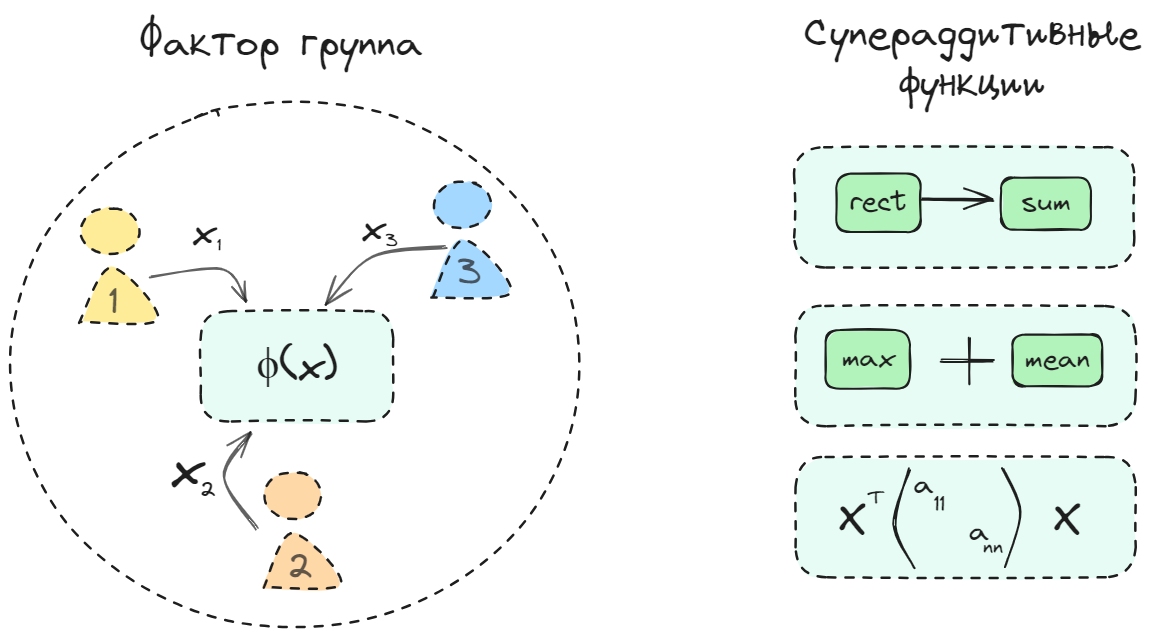
\includegraphics[width=0.5\textwidth]{assets/final/group.excalidraw.png}
%     \caption{Групповые задания}
%     \label{group_task}
% \end{figure}


Общий результат лучше исключает
случайности и может быть оценкой эффективности как отдельного педагога, так и всего преподавательского коллектива.
Тем не менее такой подход не всегда может учесть индивидуальные образовательные потребности учащихся. Одним из возможных
разрешений такой проблемы является объединение учащихся в группы для выполнения задач.

Учет коллективных эффектов
выполняется в постановках распределенной оптимизации, теории марковских полей и теоретической физике. Для анализа взаимодействия в группах малых групп используются 
ковариационные матрицы. 
